\documentclass{sig-alternate-05-2015}

\begin{document}

% DOI
\doi{}

% ISBN
\isbn{}

%Conference
%\conferenceinfo{PLDI '13}{June 16--19, 2013, Seattle, WA, USA}

%\acmPrice{\$15.00}

%
% --- Author Metadata here ---
%\conferenceinfo{Turing Scholars Class of 2016}{Austin, Texas USA}
\conferenceinfo{College of Natural Sciences, Department of Computer Science,
Building-Wide Intelligence Lab}{Austin, Texas}
%\CopyrightYear{2007} % Allows default copyright year (20XX) to be over-ridden - IF NEED BE.
%\crdata{0-12345-67-8/90/01}  % Allows default copyright data (0-89791-88-6/97/05) to be over-ridden - IF NEED BE.
% --- End of Author Metadata ---

\title{Virtour: Telepresence system for remotely-operated building tours}

\numberofauthors{5}
\author{
% 1st. author
\alignauthor
Patricio Lankenau\\
\email{pato@cs.utexas.edu}
% 2nd. author
\alignauthor
Shiqui Zang
% 3rd. author
\email{szhang@cs.utexas.edu}
\alignauthor
Jivko Sinapov
\email{jsinapov@cs.utexas.edu}
\and 
% 4th. author
\alignauthor
Matteo Leonetti
\email{m.leonetti@leeds.ac.uk}
% 5th. author
\alignauthor
Peter Stone
\email{pstone@cs.utexas.edu}
}
\date{August 14 2016}

\maketitle
\begin{abstract}
  This is my abstract
\end{abstract}

\keywords{robots, telepresence, remote control, virtual tours}

\section{Introduction}

The University of Texas at Austin has a constant stream of visitors and tours
of the beautiful campus. Of special interest to us, are the large number of
tours given at our computer science building: the Gates Dell Complex (GDC). The
tour guests range in ages and backgrounds, and tend to be prospective students
to both undergraduate and gradate programs, or visiting faculty. Unfortunately,
there is a large population of prospective students that are unable to
physically come to our campus and are thus unable to partake in the
conventional tours.

Our lab has a group of autonomous wheeled robots which can localize, navigate,
and perform tasks without human intervention for long periods of time.
Furthermore, our lab is placed in a central part of our building and is thus a
common place for tours. As such it only made sense that we utilize the platform
we have built to try to solve the aforementioned problem.

This is why we designed Virtour. Virtour is a public facing system for
teleoperated building tours. Virtour builds on the existing Building-Wide
Intelligence autonomous robot platform and is designed to keep the robots and
any humans involved safe. Through the use of modern web and robot technologies
it allows untrained public users to remotely control our robots in what we call
a virtual tour. Our system is created to balance external control abilities
while maintaining our rigorous standard of safety and security for the robots
and people involved. As such it gives the user control of what the robot is
doing, while at the same time using existing the autonomous navigation
capabilities and obstacle avoidance.

\section{Related Work}

\section{Building Wide Intelligence}

Virtour is a part of the Building Wide Intelligence (BWI) project,
which aims to develop fully autonomous mobile robots. The goal is to have these
robots be permanent inhabitants of UT's Computer Science departmental
building. BWI focuses on the intersection of Artificial Intelligence and
Robotics, and aims to create robots that are useful as research platforms, as
well service robots to help the humans in the building.

Virtour runs on the BWI segbot robot platform. The segbot robot platform
has three currently operating versions. Our last generation version 2 robots, a
version 2 with an additional Kinova arm, and our latest generation version 3
robots. Although virtour supports all three versions, it is mostly run on the
latest generation so that is what is described.

\begin{figure}
\centering
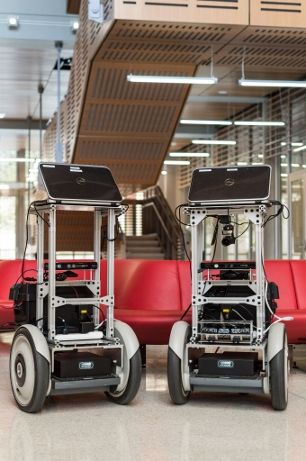
\includegraphics[height=2in]{bwi}
\caption{Two of our second generation BWI robots}
\end{figure}

\subsection{Hardware Platform}

The robot's base is a Segway Robotics Mobility Platform (RMP), which is
powered by a lithium-ion battery pack. The frame was designed in-house and
supports a wide array of sensors. For navigation, localization, and obstacle
avoidance, we use a Velodyne Puck lidar. Point clouds and RGB data is provided
by a Microsoft Kinect. Our latest generation robots also have a laser range
finder to compensate for the lidar's blind spots. The robot is equipped with a
custom-built computer which runs Ubuntu 14.04. The computer is powered by the
RMPs battery, thus removing the need for an external car battery (which was
present in our version 2 robots).  The battery life on a running robot is
approximately 6 hours.

\subsection{Software Stack}

Our robots are powered by the Robot Operating System (ROS), which provides us
with the infrastructure to run our robots as a distributed node system. ROS
also provides us with access to many community packages such as device drivers,
navigation implementations, and planning systems. Our navigation stack starts
out with the logical planner, which uses ASP to plan and describe the
environment (eg: which corridors connect with which hallways, and which doors
are open). It then moves to the logical navigator which uses the global costmap
(generated from previous laser readings, and is an adjacency grid of obstacles)
to create the navigation plan.  Finally, the local planner uses the immediate
sensor readings to send commands to the segway base and avoid any obstacles.

\section{The Web Client}

\begin{figure}
\centering
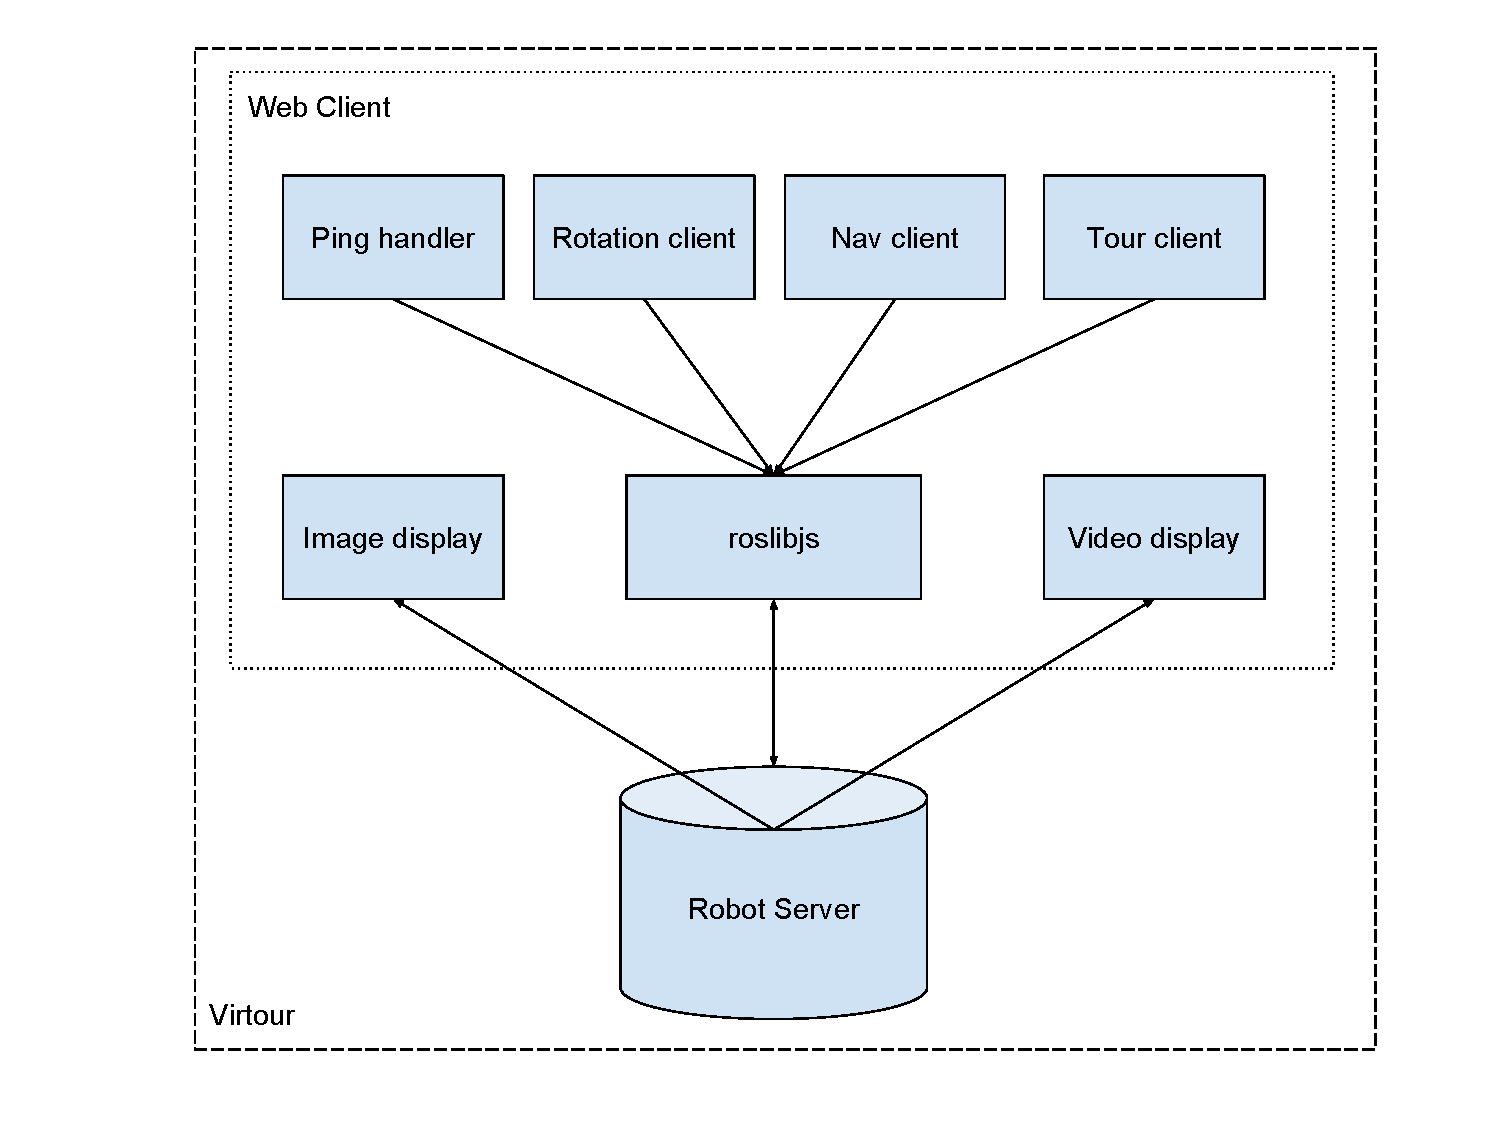
\includegraphics[height=2in]{virtour_client}
\caption{Overview of the virtour client structure and hierarchy}
\end{figure}

Virtour consists of two platforms, the user facing client, and the server
and associated software that runs on the robots. The user client is built using
web 2.0 technologies to adhere to modern web development trends and
simultaneously support as many platforms as possible. We decided to use a
web-based client because of the increasing prominence of web browsers in
people's lives. Furthermore, a web based approach means that our end-users do
not have to install any additional software to connect with or use the robots,
thus reducing the friction for trying our service.

\subsection{Modern Approach}

The website is designed to be simple and functional while still being
aesthetically pleasing to end users. It uses a grid system, powered by
Bootstrap 2.0, to create a fully responsive web layout. This allows us to
support any web-powered platform (eg: mobile devices, tablets, and computers)
by making the website scale and re-organize based on the specifications of the
device.

When a user first visits our website, he or she is greeted by a list of our
currently active and available robots (more on server implementation later).
From here our user can select a robot to connect to (by clicking on the robot's
name and image) to initiate a virtual tour session. Tour sessions can be either
led or spectated. Each tour can have at most one leader, but no limit on the
number of spectators. If the tour has no existing leader and tours are allowed
then a visiting user can elect to become tour leader by pressing the ``Become
Leader'' button. Upon success, it will present the user with the leader UI.

\begin{figure}
\centering
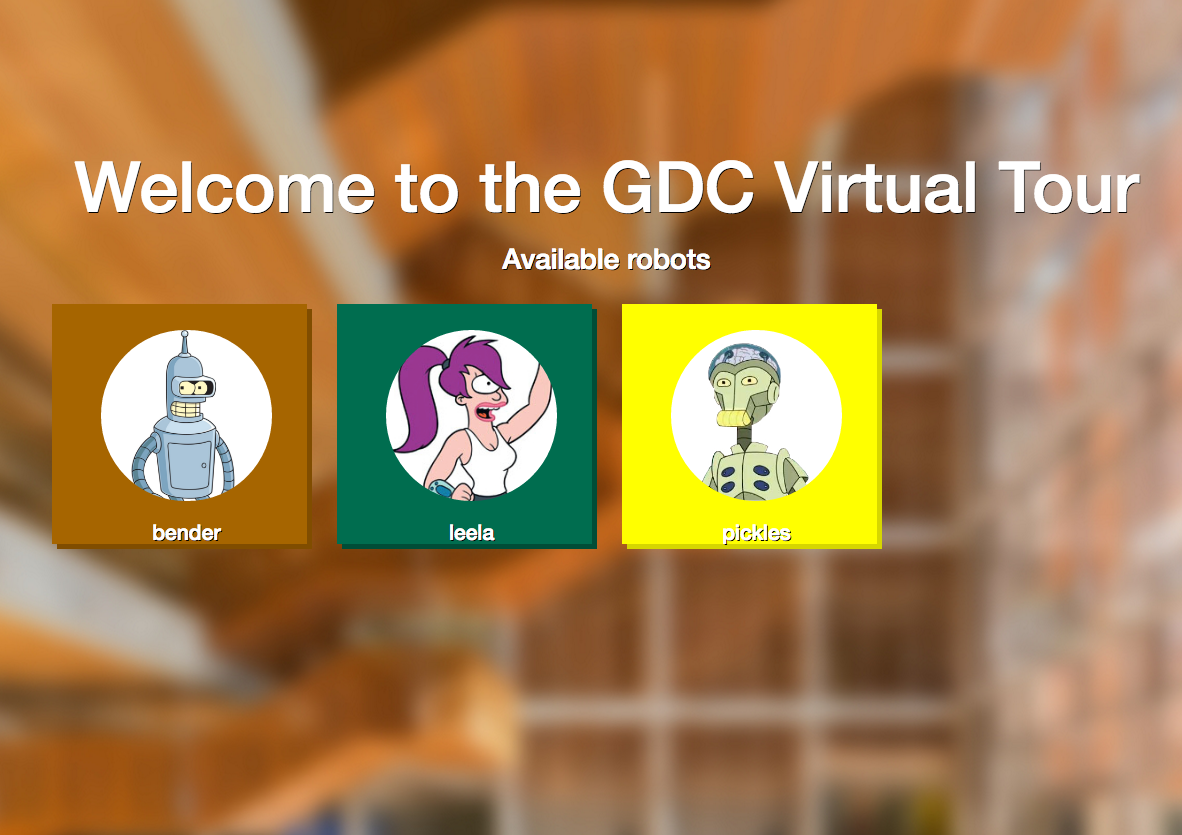
\includegraphics[height=2in]{tour_homepage}
\caption{Landing page whenever someone visits the home page}
\end{figure}

\subsection{Leader UI}

The leader UI adds a number of components to the guest UI that allow the user to
control the operations of the robot. The current list of available capabilities
is as follows

\begin{itemize}
  \item Rotate the robot's base
  \item Navigate to a room on the same floor
  \item Navigate to a door on the same floor
  \item Speak a message (using text-to-speech)
  \item Deliver a spoken message (using text-to-speech) to a location
  \item Pause and resume a robot task
  \item Move the robot's camera (on supported robots)
\end{itemize}

The user can interact with the interface to request any of the previously
mentioned tasks.

Whenever a user first connects to a robot, the web client will query the robot
for the capabilities that it has (eg: which generation robot, which cameras it
has access to, if the camera has servos, etc...) and then adapt the user
interface accordingly to support whichever robot the user is connected to.

The leader UI was developed using javascript and uses sockets to
communicate with the robot. The javascript client can interact with ROS via the
socket to make service calls, subscribe and publish to topics, as well as make
actionlib requests. Regardless of the type of the request, it is serialized and
transferred over the socket to be interpreted by the server (described in a
later section).

In order to maintain leader consistency, the leader UI will ping the server at
a known interval to ensure the leader is still connected. If the user closes
the window or the ping fails, the leader will relinquish the leader status so
other users can control robot.

For security reasons, we only allow outside parties to become leaders (and thus
have control of the robot's operations) if we explicitly enable virtual tours
on the robot. Furthermore, all leader operations that affect the robot (eg:
rotating, or navigating) require user authentication, to prevent unauthorized
sources to take control of our robots. On the client side, this means that each
user is assigned a unique identifier (valid only for the current session).
Whenever a user requests leadership, they request it for their unique
identifier. All subsequent requests are made using this identifier to ensure
that only an authorized user can control the robot.

\subsection{Guest UI}

\begin{figure}
\centering
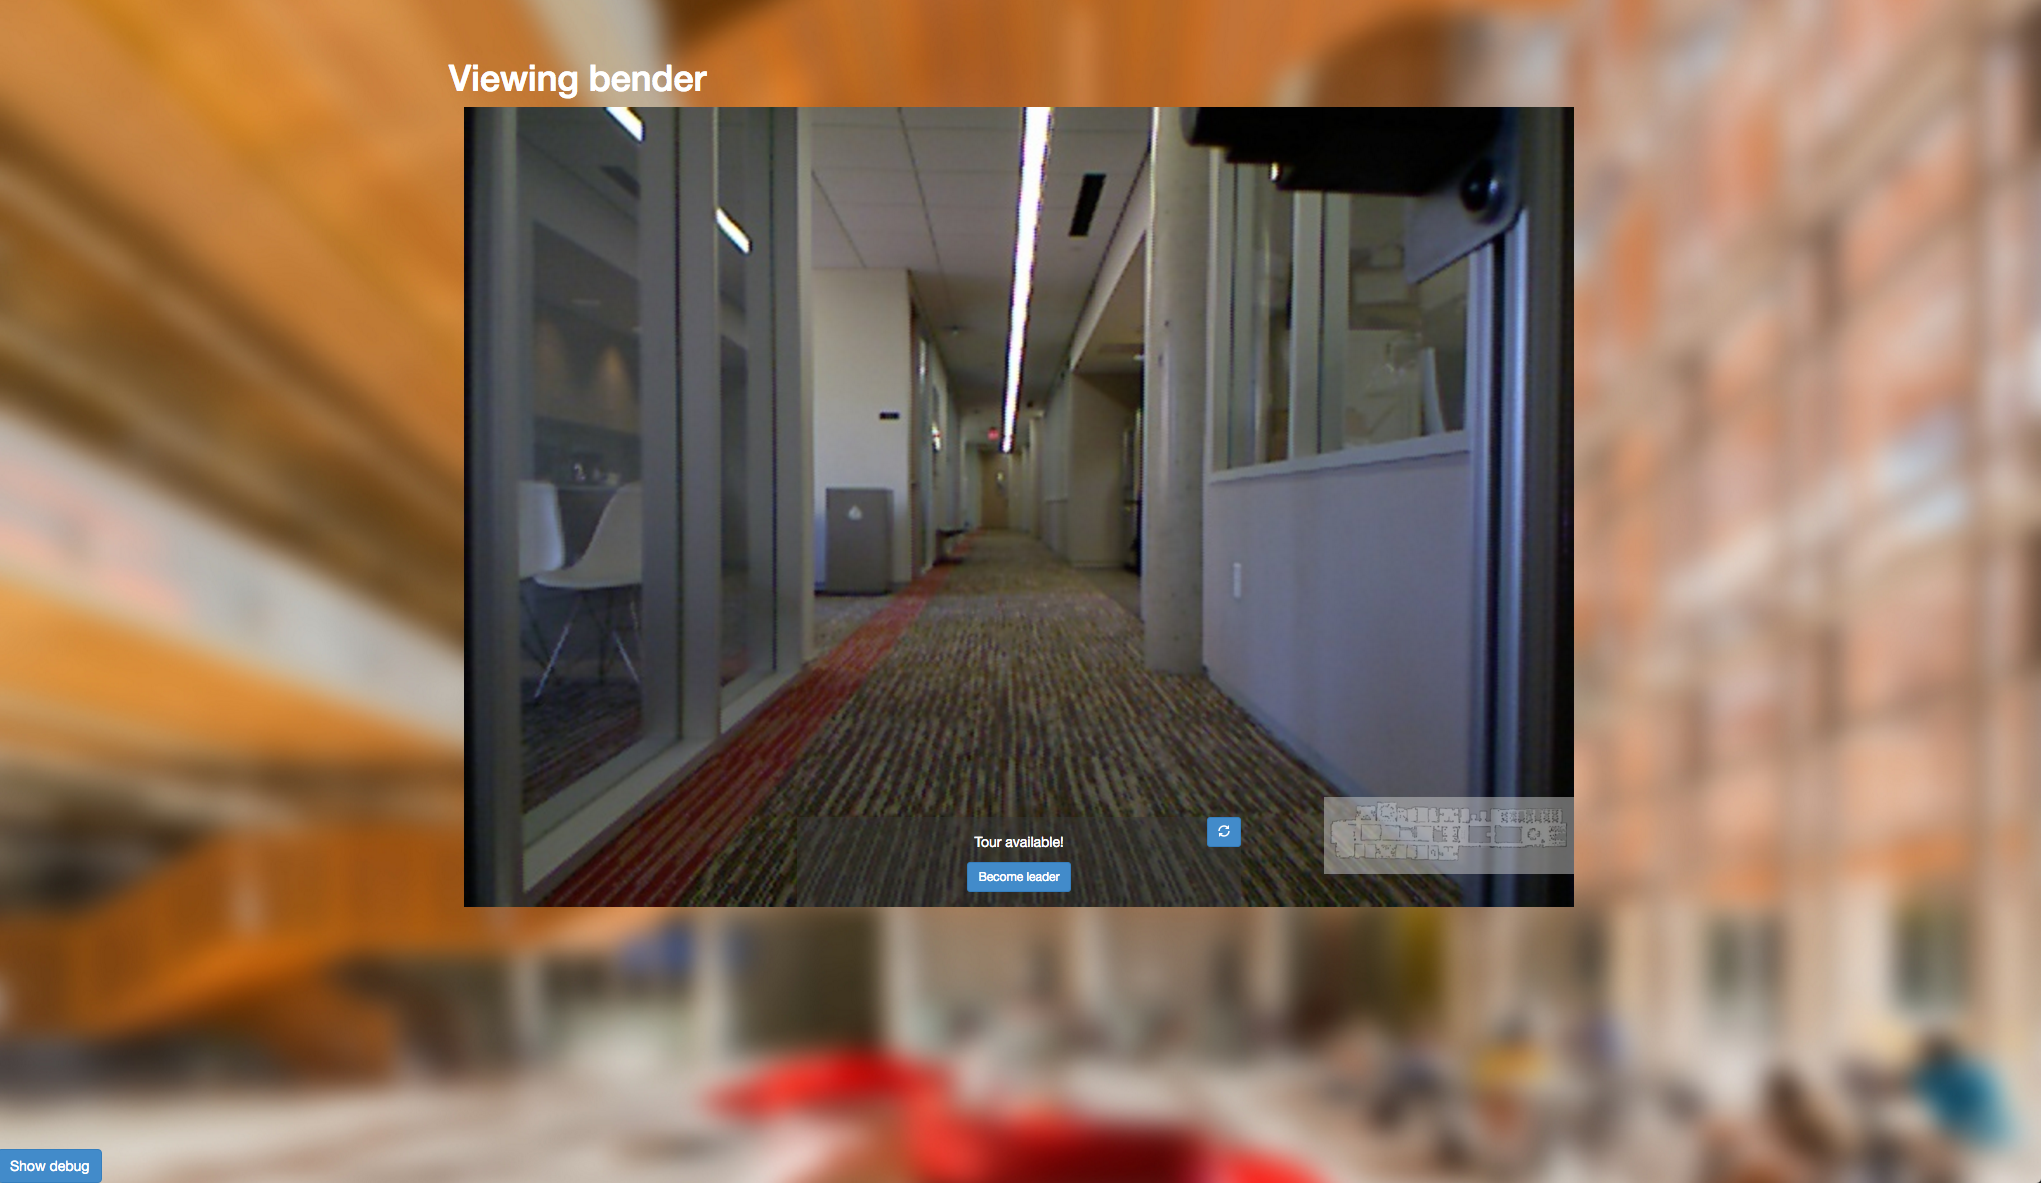
\includegraphics[height=2in]{guestUI}
\caption{What the client sees whenever they are in guest mode}
\end{figure}

The guest UI is the default interface presented to the user whenever he or she
connects to a robot. It dominated by the live stream from the robot's camera
which is shown prominently in the center. The robot's camera is placed in a
position on the robot that makes the user experience feel like a point of view
camera. This makes the experience more immersive and the tour more engaging.

Furthermore, the interface also displays a mini map of which ever floor the
robot is on, with a position marker to indicate the robot's current position.
This map is updated whenever the robot switches floors (via the elevator) to
show the most up to date map of the current floor.

Finally, the guest UI has a status box which displays whether or not a tour is
on-going, allowed, or disabled. From here the user can request to become tour
leader (if available), or wait for a tour to be available.

All our robots support the guest UI during all times we are running them, so
that users can remotely connect to the robots and experience what they are
doing.

\section{The Server}

\begin{figure}
\centering
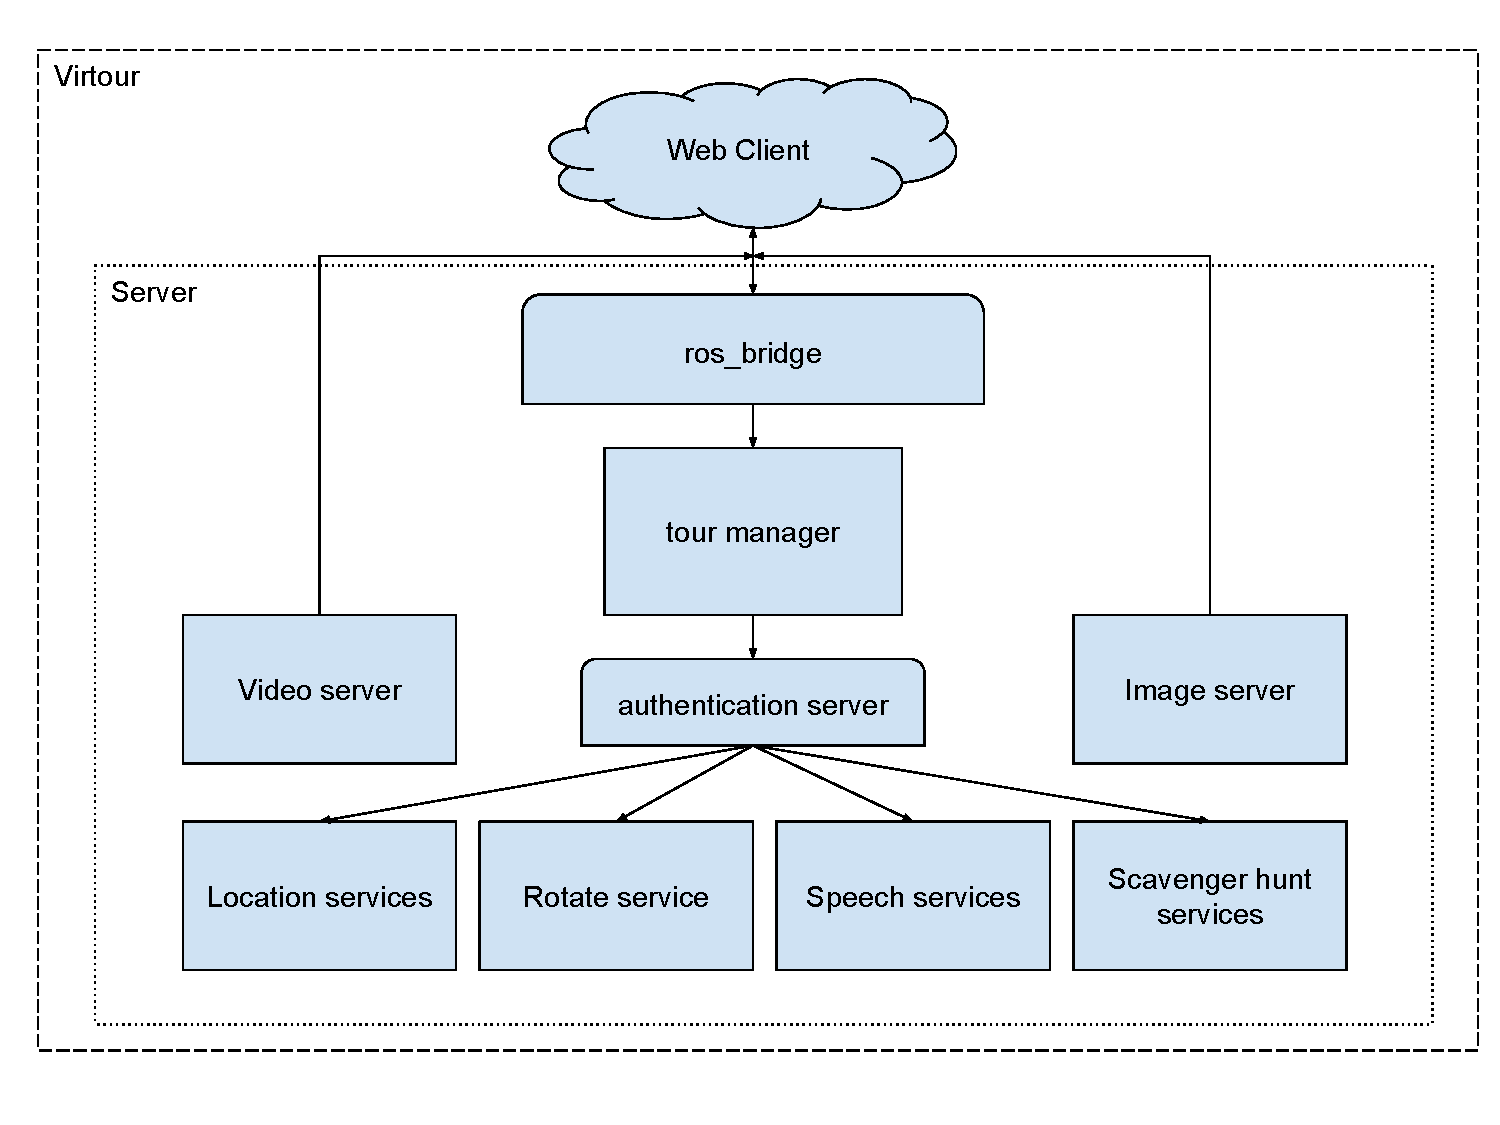
\includegraphics[height=2in]{virtour_server}
\caption{Overview of the virtour server structure and hierarchy}
\end{figure}

The server consists of a number of components which run on the physical robot
to enable the web client to perform the required operations. All communications
from the web client hit the \verb|ros_bridge| node, which then translates the
commands to ROS commands. From there, all requests are sent to the tour
manager, which will authenticate the requests (to ensure they are validly
formed and come from an accepted source) and then triage them to their
respective service providers.

\subsection{Tour Manager}

The tour manager serves the role of maintaining tour integrity and managing
active connections with all the clients that are connected to the robot. It
keeps track of an internal state machine which controls whether tours are
enabled and if so whether they are active. It will also maintain connection
with the tour leader through pings to ensure the leader remains alive. If the
leader disconnects (by closing the page) or is disconnected (missing a ping),
the tour manager will demote them and open up the tour again. The tour manager
will also grant tour leader status to clients that properly request it whenever
tours are enabled.

\subsubsection{Authentication}

Due to the open nature of virtour (anyone can access/control our robots),
security became an important factor.User authentication is done by generating a
unique identifier to each client connected (generation is done client-side).
This identifier is used to keep track of all the clients and the leader. All
requests which control robot (ie: navigating, rotating, delivering messages) go
through the authentication server. This verifies that the request is properly
created, is coming from a valid leader, and is being executed at a time when
tours are enabled. There is a 15 minute limit per leader, to avoid
a single leader taking control of the system. Finally, we always have the
option to disable tours (via the tour manager) which will immediately evict any
active leaders and restore control of the robot.

\subsubsection{Robot Control}

The server-side code powering the remote robot control consist of various
service providers which use the tour manager to authenticate requests, and then
triage them to the appropriate robot commands. For example, the rotate control
will take the rotate command (if properly authenticated) and then translate it
to raw segway base navigation commands, which is considered safe because
rotation stays within the robot's footprint so we do not need to consider
obstacle avoidance. However, obstacle avoidance is very important whenever we
are navigating to rooms or doors. For this reason, all navigation commands will
go to the logical planner in the form of ASP goals. For example a request to
navigate to a specific office will be turned into an ASP goal such that it is
impossible for the robot to not be in that location. The navigation and
planning stack then take over and will perform the planning and navigation
required to accomplish the goal.

\subsection{IP management}

In order to manage the IP addresses of all the robots, we created smallDNS
(small multi-agent locally listable DNS). SmallDNS keeps track of the IP
addresses of each of the robots (which are assigned via DHCP and are thus
variable). Furthermore, it also keeps track of which robots are available and
running via series of pings. This means that the end user does not need to
worry about the IPs of the robots or which ones are alive. So when the user
visits the home page (figure 3), they will see the list of currently active
robots and will be able to connect to each without having to know the IP
address.

SmallDNS consists of a simple DNS server running on our master server in the
lab, and a cronjob that runs on each of the robots. That way if the robot
detects that it has changed IP address, it will inform the server. As time
passes, the server will try to ping all the active robots to ensure that they
are still alive. SmallDNS serves the state of its IP database in json
format, which is what virtuour ultimately uses.

\section{Scavenger Hunt Integration}

\section{Conclusions}

\section{Acknowledgments}

\bibliographystyle{abbrv}
\bibliography{sigproc}  % sigproc.bib is the name of the Bibliography in this case
\end{document}
